\section{Data}

\subsection{Institutional Details}

The California Department of Transportation (Caltrans) is the department that
manages Aeronautics, Highway Transportation, Mass Transportation,
Transportation Planning, Administration, and the Equipment Service Center in
California. To outsource the labor for their highway construction projects,
Caltrans runs low-bid procurement auctions. Within the auctions, there are
typically large and small business bidders. Because small businesses have lower
economies of scale, their costs are higher compared to large businesses.

Due to the difference in costs, Caltrans grants ``bid preferences'' to the small
business bidders. Small businesses must meet three qualifications to be obtain
the Small Business Certification. The certification requires that the business
must be independently owned and operated in California, have no more than 100
employees, and over the last three tax years can only earn under \$10 million
average annual gross receipts. The benefit of the Small Business Certification
is that there is a higher probability of winning the auction.

Once all bids are submitted, the lowest bid wins the auction. However, if a
small business’s bid is within 5\% of the lowest bid, they win the auction and
are awarded the contract for construction. While the 5\% discount is used to
determine the winner, it is not applied to the actual amount the business is
paid for the project: Caltrans will pay the true price the winner bid.

\subsection{Data Overview}

% latex table generated in R 4.2.3 by xtable 1.8-4 package
% Sun May  7 12:37:20 2023
\begin{table}[ht]
\centering
\begin{tabular}{lrrrr}
  \toprule
 & Mean & Standard Deviation & Minimum & Maximum \\ 
  \midrule
Bids & $9.876 \times 10^{5}$ & $3.33 \times 10^{6}$ & $4.5 \times 10^{4}$ & $5.9 \times 10^{7}$ \\ 
  Small Business Bids & $5.283 \times 10^{5}$ & $7.211 \times 10^{5}$ & $5 \times 10^{4}$ & $1.5 \times 10^{7}$ \\ 
  Large Business Bids & $1.278 \times 10^{6}$ & $4.19 \times 10^{6}$ & $4.5 \times 10^{4}$ & $5.9 \times 10^{7}$ \\ 
  Number of Bidders & 5.759 & 3.155 &   2 &  20 \\ 
  Business types present & 1.673 & 0.4696 &   1 &   2 \\ 
  Engineer's Estimates & $9.475 \times 10^{5}$ & $3.756 \times 10^{6}$ & $9.1 \times 10^{4}$ & $6 \times 10^{7}$ \\ 
  Workdays & 94.06 & 155.9 &   8 & $1.4 \times 10^{3}$ \\ 
   \bottomrule
\end{tabular}
\caption{Summary statistics for subset of auctions with 2 or more bidders.} 
\end{table}


For the summary statistics, we excluded auctions with only one bidder. All statistics
are from that subset of the data.
The mean small business bid was \$528,318, and the mean large business bid
was \$1,277,866.
A possible explanation for this discrepancy is that small businesses were not
bidding on the largest contracts, perhaps because they do not have the
capacity for multi-million dollar projects. The smaller standard deviation of
small business bids also supports this theory.

In addition, out of 669 auctions in total, there were 5.8 bidders in
each auction on average, and the average bid was \$987,619.
The ``business types present'' statistic refers to whether small business,
large business, or both types of bidders participated in each auction. The
mean of 1.64 suggests that the majority of auctions had both types participating.

We calculated the winning bids and saw that on average, the winning bid was
\$52,629 lower than the state's cost estimate. CalTrans was therefore able to
reduce costs compared to their own engineers' estimates by running auctions for
procurers. Auction theory would suggest that the greater the number of bidders,
the more the cost will be driven down for the procurer due to competition.
There could potentially be a winner's curse if it is impossible to drive costs
much lower than the estimate, but we cannot determine that from this data alone.
Furthermore, the standard deviation of the differences is quite high
at almost \$1 million, and there are some cases where Caltrans
is forced to pay a premium over their estimate - it is unclear if this
represents unreliability by the engineers making the estimates,
or an underlying dynamic of the auction process.

\subsection{Bidding Behavior}

%\lstinputlisting[firstline=38, lastline = 47]{./code/data.R}

\subsubsection{Kernel Density Estimation}

First we estimated the true distribution of bids for large and
small businesses using kernel density estimation with a bandwidth
selected via leave-one-out cross-validation.
Kernel density estimation relies on the second derivative of the
density function, and will as a result tend to overestimate peaks and
underestimate valleys. We can see that in this plot, where
the density estimate is much higher than the first peak.

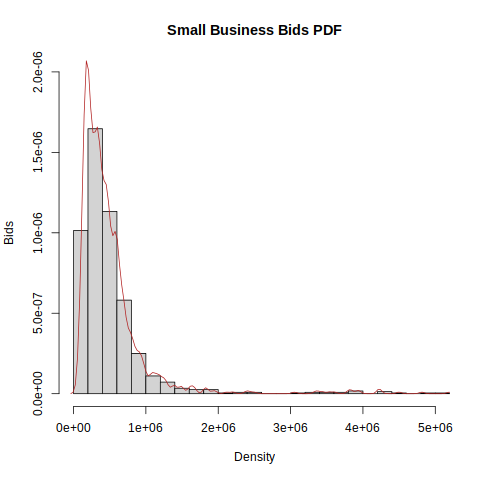
\includegraphics[scale=0.5]{imgs/sb-pdf.png}
%\begin{figure}[htb!]
%    \centering
%    %\textbf{Your title}\par\medskip
%    \begin{subfigure}[b]{.55\textwidth}
%      \centering
%      %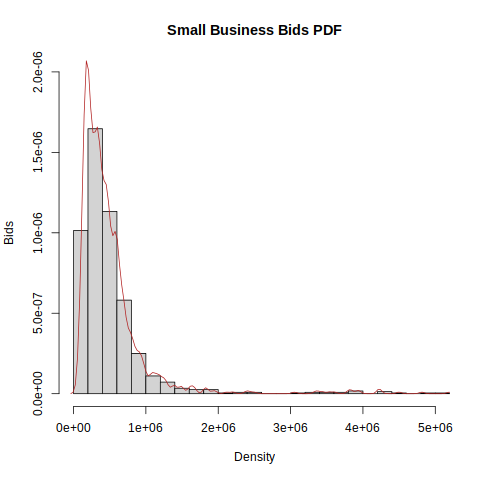
\includegraphics[width=.4\linewidth]{imgs/sb-pdf.png}
%      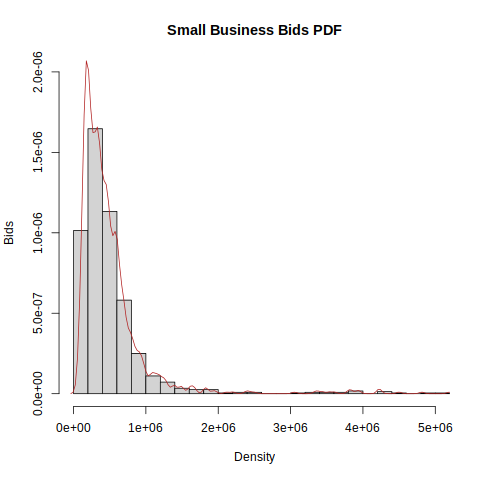
\includegraphics[width=1\linewidth]{imgs/sb-pdf.png}
%      %\caption{A subfigure}
%      \label{fig:sub1}
%    \end{subfigure}%
%
%    \begin{subfigure}[b]{.55\textwidth}
%      \centering
%      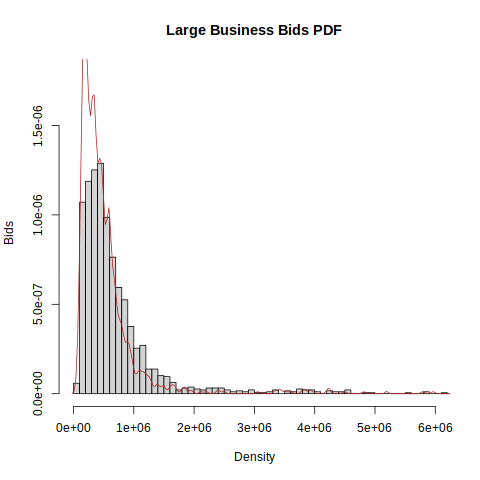
\includegraphics[width=1\linewidth]{imgs/lb-pdf.png}
%      \label{fig:sub2}
%    \end{subfigure}%
%    \caption{PDF of the bids split up by bidder size classification}
%    \label{fig:bid-pdfs}
%\end{figure}
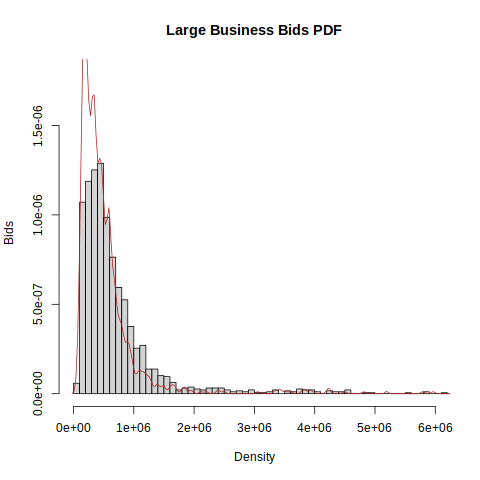
\includegraphics[scale=0.5]{imgs/lb-pdf.png}

The large business bids do have a longer tail, which reflects that
they are more able to take on projects with a large cost than
the smaller businesses.
There are also clusters in the bid frequencies, which we can see in
the spikes in the KDEs of the PDFs. One possible explanation is that the distribution
of bids is not perfectly uniform, but instead clusters because projects
can be grouped into similar size categories, and because people generally prefer
to deal with round numbers when it comes to money.
Many more projects will receive bids at \$1 million than at
\$1,010,000.
It is also possible that clusters are simply an artifact of the KDE process,
but we used biased cross-validation to select the bandwidths, which should
not undersmooth the data.

Because of the data's skew, we applied a log transformation to
normalize the data. Log scaling data can effectively compress
very wide ranges down, so that extreme bids are proportionally less
large. Consequently, the goal of this transformation was to
provide a better visualization of the long tail in our data.
\begin{figure}[ht!]
    \centering
    %\textbf{Your title}\par\medskip
    \begin{subfigure}{.5\textwidth}
      \centering
      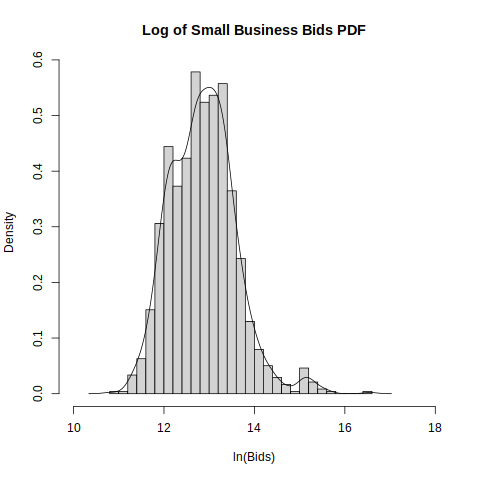
\includegraphics[scale=0.5]{imgs/log-sb-pdf.png}
      \caption{PDF of the log-bids by small businesses}
    \end{subfigure}%
    ~ % note that the subfigures will appear on top of each other if there is a breaking space between them
    \begin{subfigure}{.5\textwidth}
      \centering
      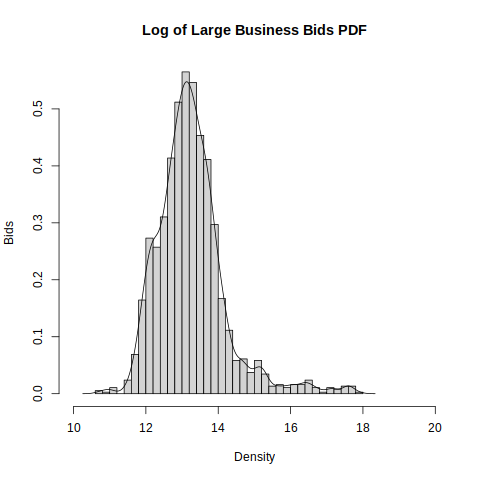
\includegraphics[scale=0.5]{imgs/log-lb-pdf.png}
      \caption{PDF of the log-bids excluding small businesses}
    \end{subfigure}%
    %\caption{PDF of the bids split up by bidder size classification}
    \label{fig:bid-pdfs}
\end{figure}
This reveals a very slight bimodal peak around bids of about \$3 million
$(\exp(15))$, which might be a common project cost.
The larger businesses look to have a very similar distribution, but just have
a higher mean, and their tail also extends further up to bids of around \$7-8
million.

% \newpage
We also plotted the CDFs to see patterns in the bid sizes between
the two types of bidders. The smaller average bids of
the small businesses are very clear in this plot, as the line is strictly
greater than the large businesses' estimated CDF.
\begin{figure}[htb!]
    \centering
    %\textbf{Your title}\par\medskip
    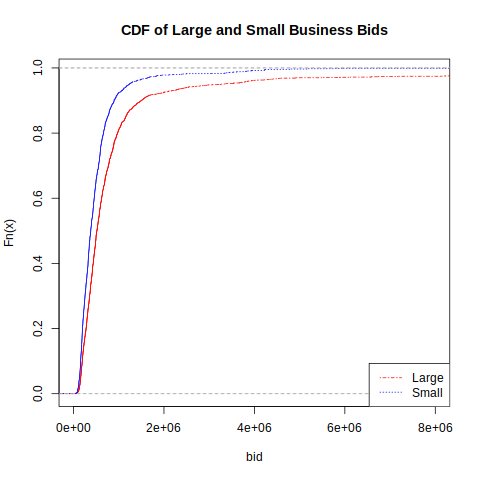
\includegraphics[scale=0.6]{imgs/cdf.png}
    %\caption{CDF of bids, split by firms deemed small businesses or not}
\end{figure}
Lastly, we plotted the CDF of the bid-estimate ratio for only small and
large businesses. Although the above plot showed the distribution of large
business bids had a much longer tail than small businesses, they generally
appear to bid a similar ratio of the estimate. This also suggests that
large businesses are taking on bigger projects, because when costs are
higher (where estimate is related to the business's true cost), they
bid higher just as small businesses do. It also is interesting that because of the
5\% rule, small businesses could theoretically `overbid,' but they are also
bidding at the same ratio of the estimate. This is likely because they have less
economies of scale and want to remain as competitive as possible, even with the
5\% rule.
\begin{figure}[htb!]
    \centering
    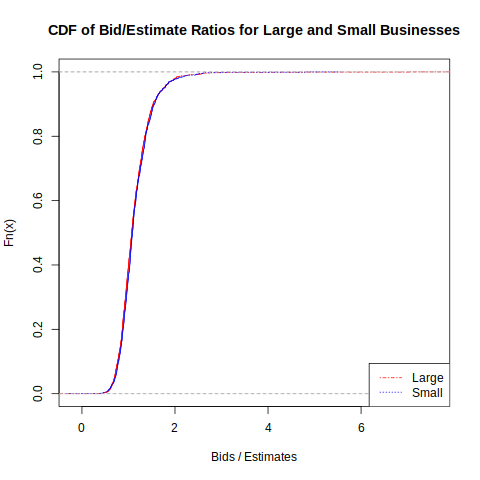
\includegraphics[scale=0.6]{imgs/cdf-bidest.png}
    %\caption{CDF of bids, split by firms deemed small businesses or not}
\end{figure}

\newpage
\subsubsection{Regressions}

To better understand the bidding behavior of business, we ran regressions on
bidders, engineer’s estimate, and work days. Bidders is how many bidders there
were for a certain project, engineer’s estimate is the estimate on how much a
professional believes the project costs, and work days is how long the project
will take. We ran regressions on all businesses, small businesses only, and
large businesses only.
The first regression including both small and large businesses gave the equation:
\[
\text{Bids} = 222576 - 18609 \text{\# Bidders} + 0.8493 \text{Estimate} + 718 \text{Workdays}
\]
The regressions on a subset gave:
\[
\begin{aligned}
\text{Bids} &= 136254 - 16423 \text{\# Bidders} + 0.9469 \text{Estimate} + 149 \text{Workdays} \\
\text{Bids} &= 178043- 20918 \text{\# Bidders} + 0.8396\text{Estimate} + 1370 \text{Workdays}
\end{aligned}
\]
In addition, below we  have included the regression tables for further analysis.
\begin{center}
% latex table generated in R 4.2.2 by xtable 1.8-4 package
% Tue Feb 21 21:12:15 2023
\begin{table}[ht]
\begin{tabular}{rrrrr}
  \toprule
 & Estimate & Std. Error & t value & Pr($>$$|$t$|$) \\ 
  \midrule
(Intercept) & 224239.4332 & 32012.8642 & 7.00 & 0.0000 \\ 
  num\_bidders & -18815.3332 & 4617.4432 & -4.07 & 0.0000 \\ 
  Estimate & 0.8494 & 0.0041 & 205.05 & 0.0000 \\ 
  WorkDays & 715.9631 & 99.6008 & 7.19 & 0.0000 \\ 
   \bottomrule
\end{tabular}
\end{table}
% latex table generated in R 4.2.2 by xtable 1.8-4 package
% Tue Feb 21 21:12:15 2023
\begin{table}[ht]
\begin{tabular}{rrrrr}
  \toprule
 & Estimate & Std. Error & t value & Pr($>$$|$t$|$) \\ 
  \midrule
(Intercept) & 224239.4332 & 32012.8642 & 7.00 & 0.0000 \\ 
  num\_bidders & -18815.3332 & 4617.4432 & -4.07 & 0.0000 \\ 
  Estimate & 0.8494 & 0.0041 & 205.05 & 0.0000 \\ 
  WorkDays & 715.9631 & 99.6008 & 7.19 & 0.0000 \\ 
   \bottomrule
\end{tabular}
\end{table}
% latex table generated in R 4.2.2 by xtable 1.8-4 package
% Tue Feb 21 21:12:15 2023
\begin{table}[ht]
\begin{tabular}{rrrrr}
  \toprule
 & Estimate & Std. Error & t value & Pr($>$$|$t$|$) \\ 
  \midrule
(Intercept) & 224239.4332 & 32012.8642 & 7.00 & 0.0000 \\ 
  num\_bidders & -18815.3332 & 4617.4432 & -4.07 & 0.0000 \\ 
  Estimate & 0.8494 & 0.0041 & 205.05 & 0.0000 \\ 
  WorkDays & 715.9631 & 99.6008 & 7.19 & 0.0000 \\ 
   \bottomrule
\end{tabular}
\end{table}

\end{center}

The above tables show the output of three regressions of the
number of bidders, estimated cost, and workdays spent on the job,
on the procurement bids.
The results of this regression are as we expected. The negative sign on bidders
is consistent with the theory, because with more bidders in a
particular auction, it drives down the price of the bid.
Similarly, as the engineer’s estimate increases, the bid should
increase because there is a higher cost for the project; and as work days
increase, so should the bid because projects that take longer become more expensive.

The results for small businesses also have the same signs as we expected, for
the same reasons as above. The only difference in this regression is the degree
to which work days
influences the bid. The coefficient for the regression with only small business
bidders is 154.3 compared with 716 for the regression including all businesses.
This might indicate that number of work days does not increase the bid as much
because smaller businesses might not be able to handle the cost of larger
projects that require more time and capital. Therefore, they can’t bid as high.

A notable difference in the final regression, which is limited
to businesses that tend to be larger, is the greater coefficient
for work days, such that there is
a much larger coefficient on work days for large business bidders. This can be
explained by the fact that large businesses can handle the higher costs of
lengthier projects. Their economies of scale allow for them to afford projects
that require more time and capital. Because of this, they are more likely
to pursue such projects and can bid higher for them.

